\chapter{Численный эксперимент}

В этой главе мы исследуем свойство нетранзитивности на реальных данных. Проведем численный эксперимент при $a = d$, $b = c$ (для простоты анализа).
То есть одна стратегия закрывалась в плюс на таком же проценте, как и другая в минус, и наоборот. Эксперимент будем проводить на акциях Сбербанка за 2017, 2018, 2019, 2020, 2021 (ticker = SBER)$^{[3]}$.
\section{Описание эксперимента}

Будем считать, что одна стратегия лучше другой, если она чаще дает больший результат. Поэтому наша цель, подтвердить, что приведенные ранее соотношения для стратегий будут выполняться. Для агрегирования данных будем использовать язык Python и библиотеку Pandas. Код будет приведен в следующей главе.
\smallskip
\smallskip

Результаты приведем в таблицах: по строкам укажем всевозможные исходы (их 9 штук), по столбцам обозначим годы. В пересечении строк и столбцов укажем процент, соответсвующий кажому исходу по годам.
\smallskip
\smallskip

Для первого эксперимента $a = d = 0.6$, $b = c = 0.3$. Результат:

\begin{table}[!ht]
\centering
\begin{tabular}{|l|l|l|l|l|l|}
\hline
     & 2017 & 2018 & 2019 & 2020 & 2021 \\ \hline
    s1 > s2 & 36.9 & 31.9 & 32.9 & 36.8 & 39.4 \\ \hline
    \rowcolor{blue}s1 > s3 & 65.5 & 63.0 & 63.9 & 66.8 & 74.3 \\ \hline
    \rowcolor{blue}s2 > s1 & 63.1 & 68.1 & 67.1 & 63.2 & 60.6 \\ \hline
    s2 > s3 & 29.0 & 31.1 & 31.3 & 30.0 & 35.0 \\ \hline
    s3 > s1 & 34.5 & 37.0 & 36.1 & 33.2 & 25.7 \\ \hline
    \rowcolor{blue}s3 > s2 & 67.1 & 59.4 & 66.7 & 61.6 & 62.4 \\ \hline
    s1 == s2 & 0.0 & 0.0 & 0.0 & 0.0 & 0.0 \\ \hline
    s1 == s3 & 0.0 & 0.0 & 0.0 & 0.0 & 0.0 \\ \hline
    s2 == s3 & 4.0 & 9.4 & 2.0 & 8.4 & 2.7 \\ \hline
    Количество дней & 252 & 254 & 252 & 250 & 226 \\ \hline
\end{tabular}
\end{table}

\textbf{Вывод:} за все годы наблюдается эффект нетранзитивности. Из таблицы видно, что $s_2 > s_1$ (действительно примерно в $2 \over 3$ случаев) и  $s_1 > s_3$ (также примерно в $2 \over 3$ случаев), но соотношение, что $s_2 > s_3$  является неверным.
\smallskip
\smallskip

 Далее возьмем $a = d = 0.4$, $b = c = 0.2$. Результат:
 \begin{table}[!ht]
    \centering
    \begin{tabular}{|l|l|l|l|l|l|}
    \hline
         & 2017 & 2018 & 2019 & 2020 & 2021 \\ \hline
        s1 > s2 & 40.1 & 35.0 & 38.1 & 38.4 & 42.0 \\ \hline
        \rowcolor{blue}s1 > s3 & 63.9 & 58.3 & 63.9 & 64.8 & 68.6 \\ \hline
        \rowcolor{blue}s2 > s1 & 59.9 & 65.0 & 61.9 & 61.6 & 58.0 \\ \hline
        s2 > s3 & 23.8 & 23.2 & 25.8 & 26.4 & 26.5 \\ \hline
        s3 > s1 & 36.1 & 41.7 & 36.1 & 35.2 & 31.4 \\ \hline
        \rowcolor{blue}s3 > s2 & 59.1 & 53.1 & 65.5 & 54.0 & 70.4 \\ \hline
        s1 == s2 & 0.0 & 0.0 & 0.0 & 0.0 & 0.0 \\ \hline
        s1 == s3 & 0.0 & 0.0 & 0.0 & 0.0 & 0.0 \\ \hline
        s2 == s3 & 17.1 & 23.6 & 8.7 & 19.6 & 3.1 \\ \hline
        Количество дней & 252 & 254 & 252 & 250 & 226 \\ \hline
    \end{tabular}
\end{table}

\textbf{Вывод:} при изменении параметров второй и третьей стратегии эффект нетранзитивности сохраняется.
\smallskip
\smallskip

 Далее возьмем $a = d = 0.5$, $b = c = 0.25$. Результат:
 \begin{table}[!ht]
    \centering
    \begin{tabular}{|l|l|l|l|l|l|}
    \hline
         & 2017 & 2018 & 2019 & 2020 & 2021 \\ \hline
        s1 > s2 & 36.1 & 32.7 & 36.1 & 37.2 & 43.8 \\ \hline
        \rowcolor{blue}s1 > s3 & 65.9 & 59.4 & 62.7 & 66.0 & 71.2 \\ \hline
        \rowcolor{blue}s2 > s1 & 63.9 & 67.3 & 63.9 & 62.8 & 56.2 \\ \hline
        s2 > s3 & 29.8 & 26.8 & 27.0 & 28.8 & 27.4 \\ \hline
        s3 > s1 & 34.1 & 40.6 & 37.3 & 34.0 & 28.8 \\ \hline
        \rowcolor{blue}s3 > s2 & 60.3 & 58.7 & 69.8 & 60.0 & 69.0 \\ \hline
        s1 == s2 & 0.0 & 0.0 & 0.0 & 0.0 & 0.0 \\ \hline
        s1 == s3 & 0.0 & 0.0 & 0.0 & 0.0 & 0.0 \\ \hline
        s2 == s3 & 9.9 & 14.6 & 3.2 & 11.2 & 3.5 \\ \hline
        Количество дней & 252 & 254 & 252 & 250 & 226 \\ \hline
    \end{tabular}
\end{table}

\textbf{Вывод:} при изменении параметров второй и третьей стратегии эффект нетранзитивности сохраняется.

\newpage
Последний эксперимент: $a = d = 2$, $b = c = 1$. Результат:

\begin{table}[!ht]
    \centering
    \begin{tabular}{|l|l|l|l|l|l|}
    \hline
         & 2017 & 2018 & 2019 & 2020 & 2021 \\ \hline
        s1 > s2 & 25.4 & 27.6 & 25.0 & 26.4 & 28.3 \\ \hline
        \rowcolor{blue}s1 > s3 & 69.8 & 74.4 & 71.8 & 70.8 & 70.8 \\ \hline
        \rowcolor{blue}s2 > s1 & 74.2 & 72.4 & 75.0 & 73.6 & 71.7 \\ \hline
        \rowcolor{blue}s2 > s3 & 50.8 & 51.6 & 49.6 & 49.2 & 46.9 \\ \hline
        s3 > s1 & 29.8 & 25.6 & 27.8 & 29.2 & 29.2 \\ \hline
        s3 > s2 & 22.2 & 34.3 & 13.5 & 30.0 & 20.8 \\ \hline
        s1 == s2 & 0.4 & 0.0 & 0.0 & 0.0 & 0.0 \\ \hline
        s1 == s3 & 0.4 & 0.0 & 0.4 & 0.0 & 0.0 \\ \hline
        s2 == s3 & 27.0 & 14.2 & 36.9 & 20.8 & 32.3 \\ \hline
        Количество дней & 252 & 254 & 252 & 250 & 226 \\ \hline
    \end{tabular}
\end{table}

\textbf{Вывод:} при изменении параметров нетранзитивность сохраняется, только в более слабом смысле: не вероятность выигрыша больше половины, а вероятность выигрыша больше вероятности проигрыша (поскольку ничьи отнимают часть полной вероятности). Также можно заметить рост равенства стратегий $s_2$ и $s_3$.

\section{Графическая эллюстрация}
Дополнительно рассмотрим на графиках всевозможные варианты реализации стратегий $s_2$ и $s_3$ для $a = d = 0.6$, $b = c = 0.3$. Всего есть 9 всевозможных реализаций (как уже было указано ранее). Опишем их и приведем графики ниже:

\begin{enumerate}
    \item $s_2$ продажа на повышение, $s_3$ продажа на повышение (рис. 3.1)
    \item $s_2$ продажа на повышение, $s_3$ продажа на понижение (рис. 3.2)
    \item $s_2$ продажа на повышение, $s_3$ продажа в конце дня (рис. 3.3)
    \item $s_2$ продажа на понижение, $s_3$ продажа на повышение (не реализуется)
    \item $s_2$ продажа на понижение, $s_3$ продажа на понижение (рис. 3.4)
    \item $s_2$ продажа на понижение, $s_3$ продажа в конце дня (не реализуется)
    \item $s_2$ продажа в конце дня, $s_3$ продажа на повышение (не реализуется)
    \item $s_2$ продажа в конце дня, $s_3$ продажа на понижение (рис. 3.5)
    \item $s_2$ продажа в конце дня, $s_3$ продажа в конце дня (рис. 3.6)
\end{enumerate}
\smallskip

Сразу отметим, что случаи, описанные под буквами г, е, ж не реализуются. Случай, описанный под пунктом и), также не был найден для выбранных  $a, b, c, d$, но при увеличении этих значений на незначительную величину приведет также к реализации этого случая (см. рис. 6). 

\begin{center}
    \begin{figure}[h]
        \centering
        \caption{$s_2$ продажа на повышение, $s_3$ продажа на повышение}
        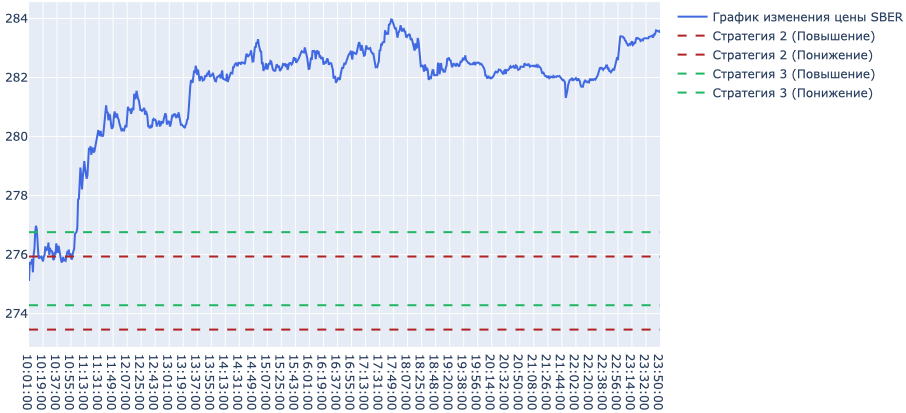
\includegraphics[keepaspectratio=true,scale=0.35]{images/chapter3/upup.png}
        
        \caption{$s_2$ продажа на повышение, $s_3$ продажа на понижение}
        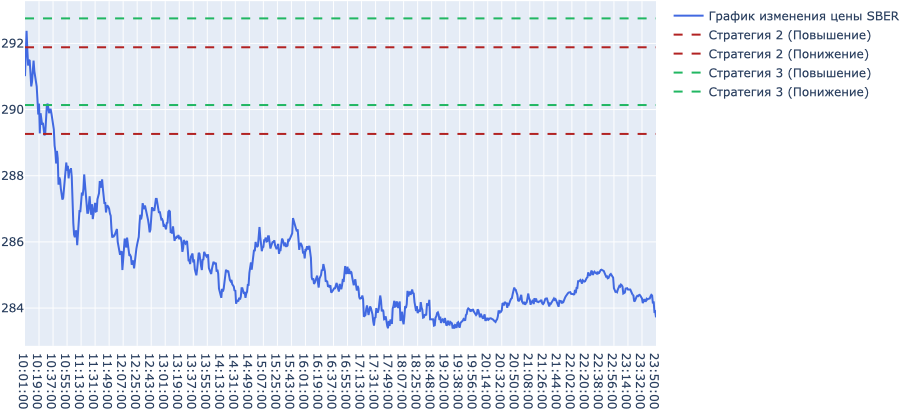
\includegraphics[keepaspectratio=true,scale=0.35]{images/chapter3/updown.png}
        
        \caption{$s_2$ продажа на повышение, $s_3$ продажа в конце дня}
        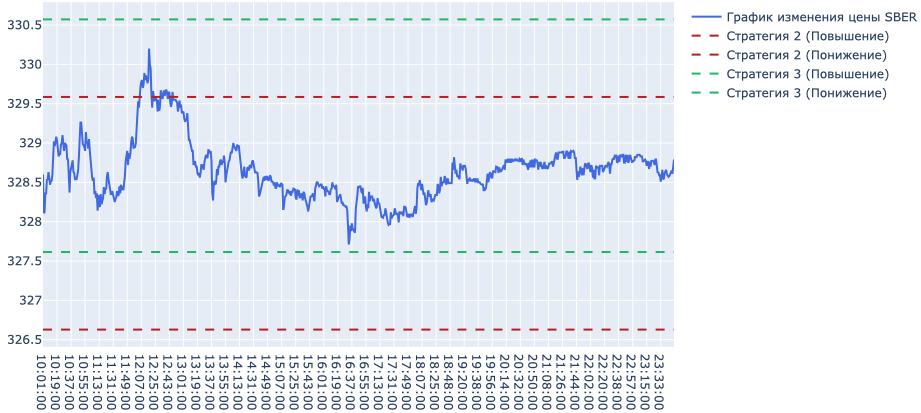
\includegraphics[keepaspectratio=true,scale=0.35]{images/chapter3/upzero.png}
    \end{figure}
\end{center}


Здесь дополнительно отмечу, что все графики были построены на тех же данных по акциям Сбербанка (ticker = SBER) за 2017, 2018, 2019, 2020, 2021. Синим цветом обозначено изменение стоимости акции в течение торгового дня(данные были взяты поминутно). Красные пунктирные линии обозначает границы продажи для стратегии $s_2$, зеленые пунктирные линии обозначают границы продажи для стратегии $s_3$. Посмотрим оставшиеся графики:

\begin{center}
    \begin{figure}[h]
        \centering
        \caption{$s_2$ продажа на понижение, $s_3$ продажа на понижение}
        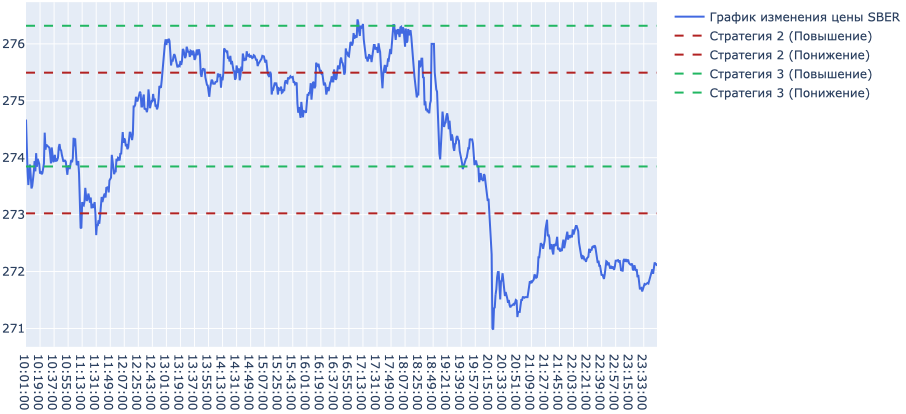
\includegraphics[keepaspectratio=true,scale=0.35]{images/chapter3/downdown.png}
        
        \caption{$s_2$ продажа в конце дня, $s_3$ продажа на понижение}
        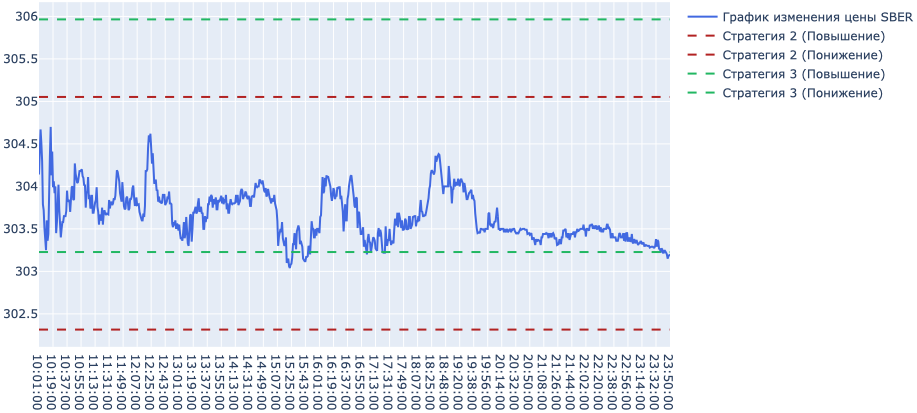
\includegraphics[keepaspectratio=true,scale=0.35]{images/chapter3/zerodown.png}
        
        \caption{$s_2$ продажа в конце дня, $s_3$ продажа в конце дня}
        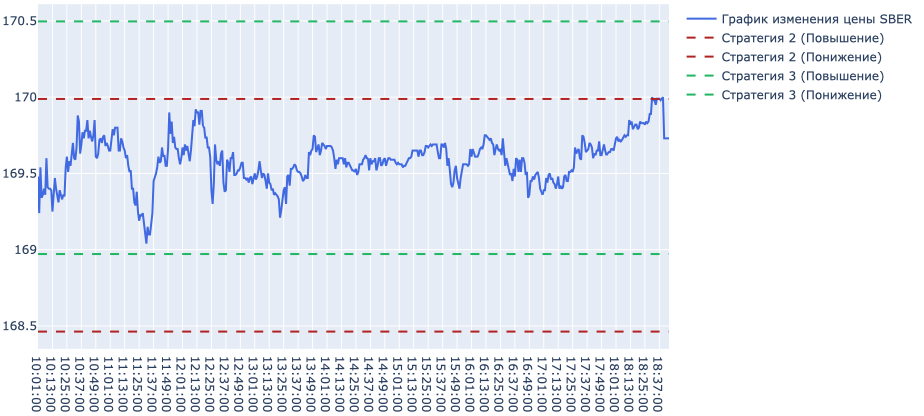
\includegraphics[keepaspectratio=true,scale=0.35]{images/chapter3/zerozero.png}
    \end{figure}
\end{center}


На этом численный эксперимент можно считать законченным. 

